\documentclass{beamer}

\usepackage{multicol}
\usepackage{clrscode3e}
\usepackage{amsmath}
\usepackage{graphicx}
\usepackage{tikz}

\newcommand{\bi}{\begin{itemize}}
\newcommand{\ii}{\item}
\newcommand{\ei}{\end{itemize}}
\newcommand{\bn}{\begin{enumerate}}
\newcommand{\en}{\end{enumerate}}
\newcommand{\set}[1]{\ensuremath{\left\{#1\right\}}}
\newcommand{\pr}[1]{\ensuremath{\mbox{Pr}\left\{#1\right\}}}
\newcommand{\flr}[1]{\ensuremath{\left\lfloor#1\right\rfloor}}
\newcommand{\ceil}[1]{\ensuremath{\left\lceil#1\right\rceil}}

\newcommand{\sect}[1]{
\section{#1}
\begin{frame}[fragile]\frametitle{#1}
}

\newcommand{\nop}[1]{}

\title{Notes on Hash Tables}
\author{Geoffrey Matthews}

\begin{document}

\begin{frame}
\maketitle
\end{frame}

\sect{Dictionary Operations}
\bi
\ii \textsc{Insert}
\ii \textsc{Search}
\ii \textsc{Delete}
\ei

\end{frame}

\sect{Hash table implementation of Dictionary}
\bi
\ii Expected search time: $O(1)$
\ii Worst case search: $O(n)$
\ei

\end{frame}

\sect{Hash table is generalization of an ordinary array}
\bi
\ii With array, the key $k$ is the position $k$ in the array.
\ii Given a key $k$, we find the element with key $k$
by \textbf{direct addressing}.
\ii Direct addressing only applicable when we can afford to
allocate an array with one position for every key.
\ei

\end{frame}

\sect{Use hash table when we don't have one position for each key}
\bi
\ii Number of keys stored is small relative to the number of possible
keys.
\ii Hash table is an array with size proportional to the number of
keys stored, not the number of possible keys.
\ii Given a key $k$, don't use $k$ to index the array.
\ii Instead, compute a function of $k$ and use that to index the
array.
\ii This function is called a \textbf{hash function}.
\ii Have to solve issue of what to do when hash function maps multiple
keys to same table entry.
\bi\ii chaining \ii open addressing \ei

\ei

\end{frame}

\sect{Direct-address tables}
\bi
\ii Scenario:
\bi
\ii Maintain a dynamic set
\ii Each element has a key drawn from a universe
$U=\{0,1,\ldots,m-1\}$ where $m$ isn't too large.
\ii No two elements have the same key.
\ei
\ii Represent by a \textbf{direct-address table}, or array, $T[0\ldots
  m-1]$:
\bi
\ii Each \textsl{slot}, or position, corresponds to a key in $U$.
\ii If there's an element $x$ with key $k$, then $T[k]$ contains a
pointer to $x$.
\ii Otherwise, $T[k]$ is empty, represented by \textsc{NIL}.
\ei
\ei

\end{frame}
\sect{Direct-address table}

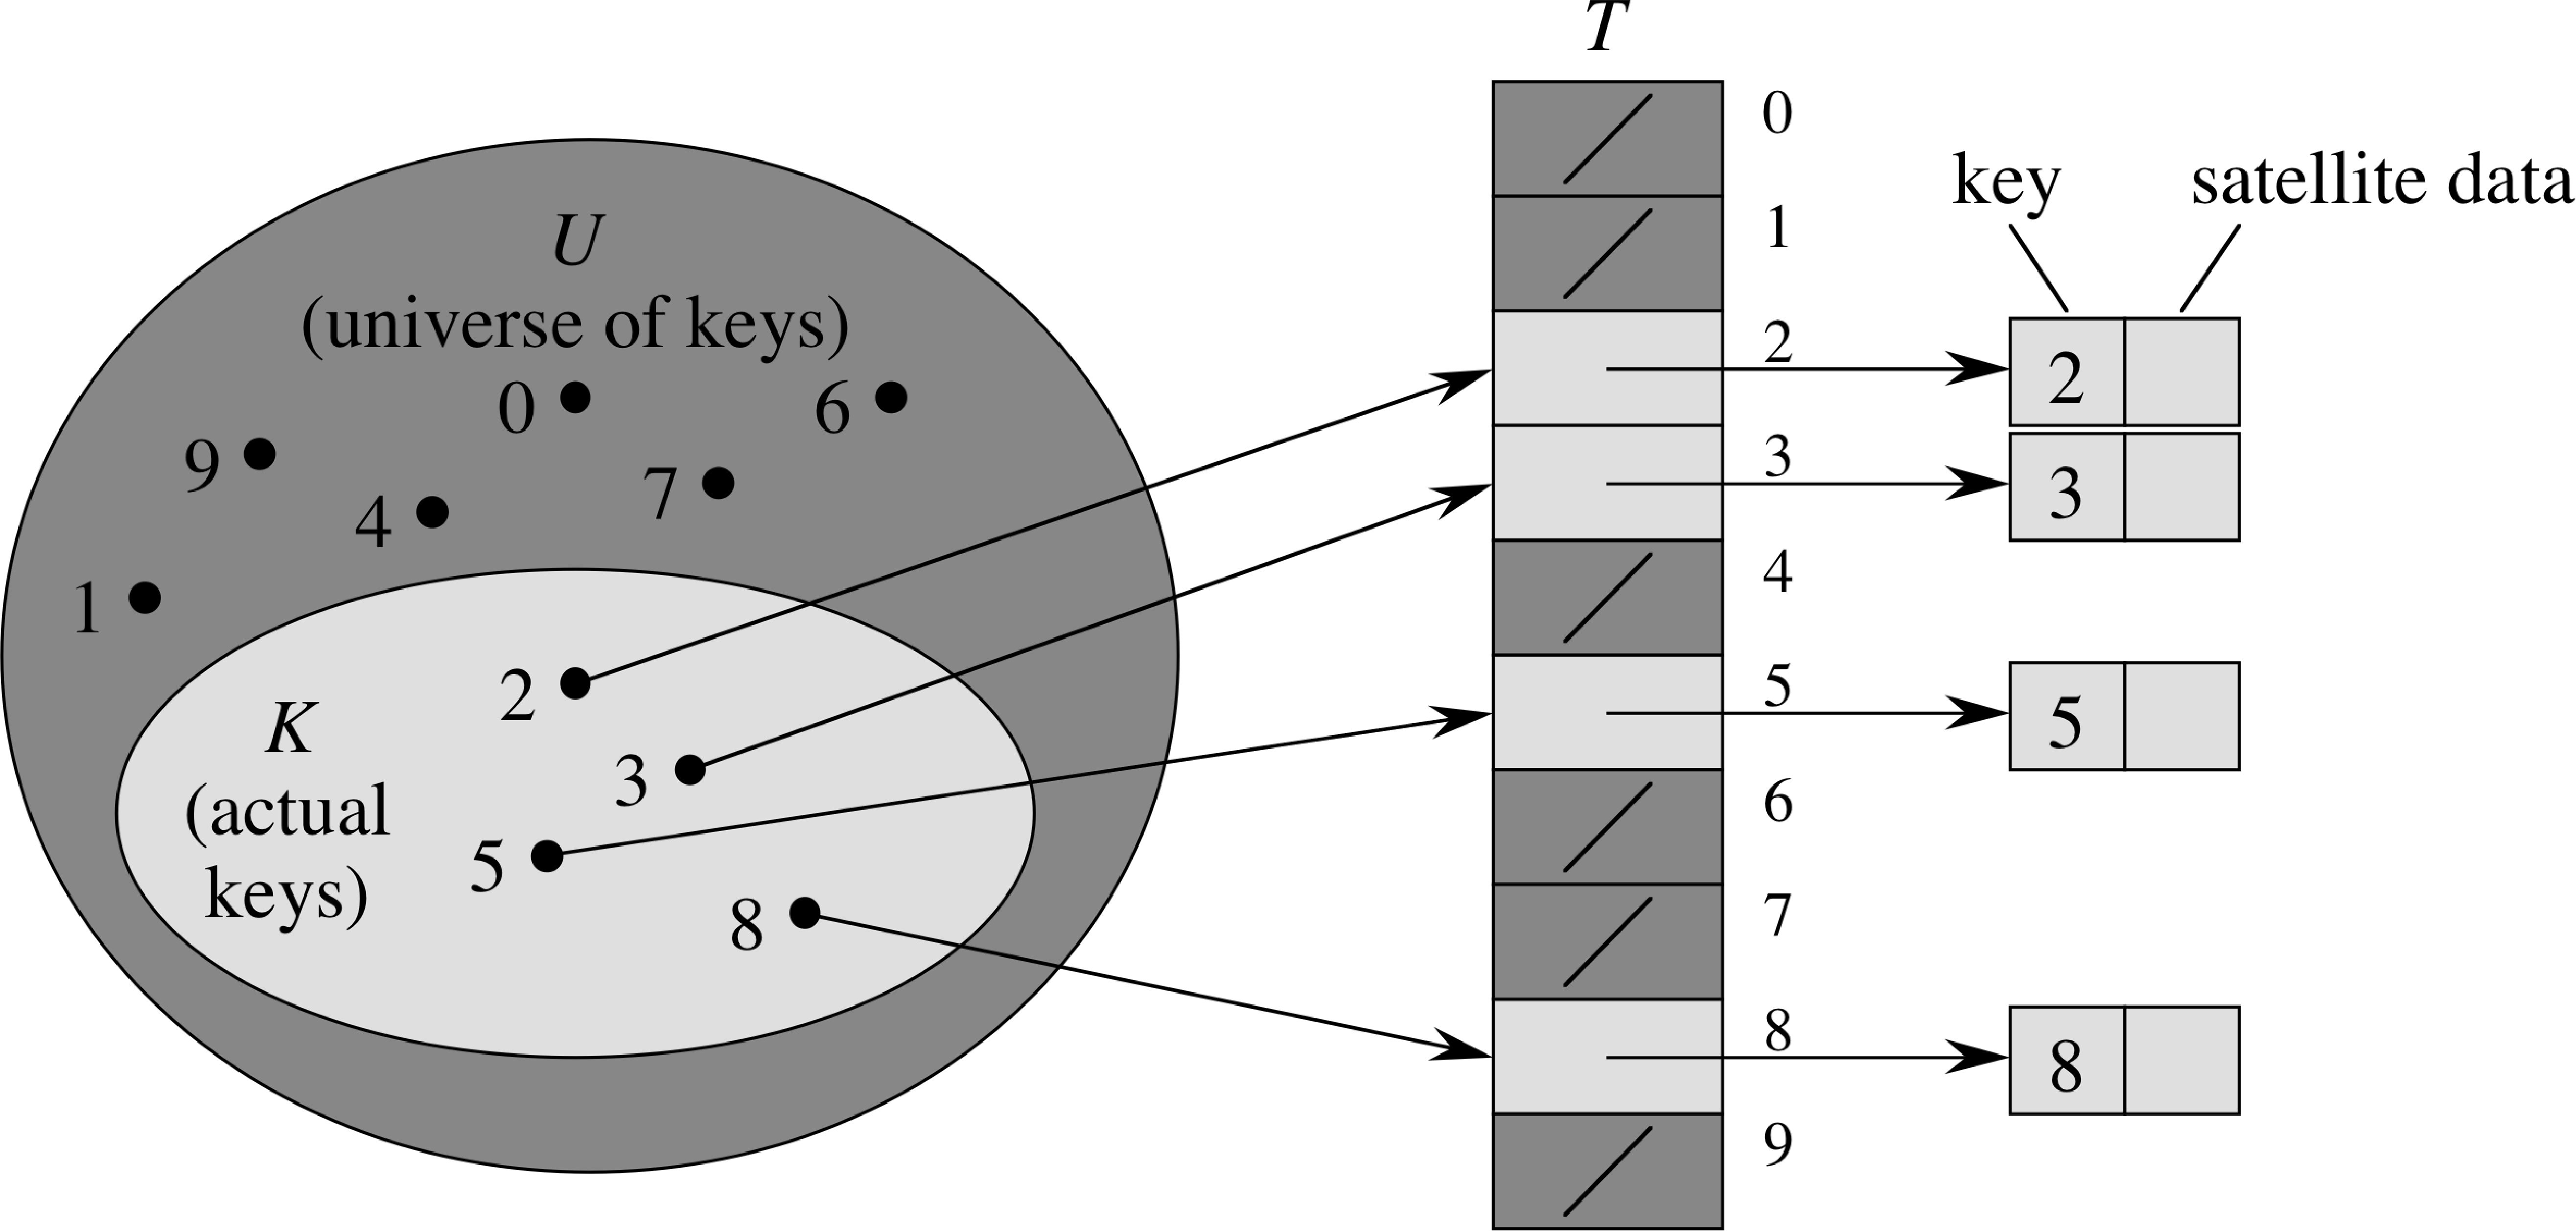
\includegraphics[width=\textwidth]{Fig-11-1.pdf}
\begin{multicols}{2}
\begin{codebox}
  \Procname{Direct-Address-Search(T,k)}
  \li \Return $T[k]$
\end{codebox}
\begin{codebox}
  \Procname{Direct-Address-Insert(T,k)}
  \li $T[key[x]] = x$
\end{codebox}
\begin{codebox}
  \Procname{Direct-Address-Delete(T,k)}
  \li $T[key[x]] = \textsc{nil}$
\end{codebox}
All operations $O(1)$.
\end{multicols}

\end{frame}

\sect{Hash tables}
\bi
\ii If $U$ is large, storing a table of size $|U|$ is impractical.
\ii Often the set $K$ of keys actually used is small compared to $U$.
\bi\ii Most of the space in a direct-access table is wasted.\ei
\ii When $K$ is much smaller than $U$, a hash table requires much less
space than a direct-address table.
\ii Can reduce storage requirements to $\Theta(|K|)$
\ii Can still get $O(1)$ search time on {\em average}, but not {\em
  worst} case.
\ei

\end{frame}

\sect{Hash table idea}
\bi
\ii Instead of storing an element with key $k$ in slot $k$,
use a function $h$ and store the element in slot $h(k)$.
\ii $h$ is called a \textbf{hash function}
\ii $h: U \rightarrow \{0,1,\ldots,m-1\}$
\ii $m \ll |U|$
\ii $h(k)$ is a legal slot number in $T$
\ii We say $k$ {\em hashes} to $h(k)$
\ei

\end{frame}

\sect{Collisions}

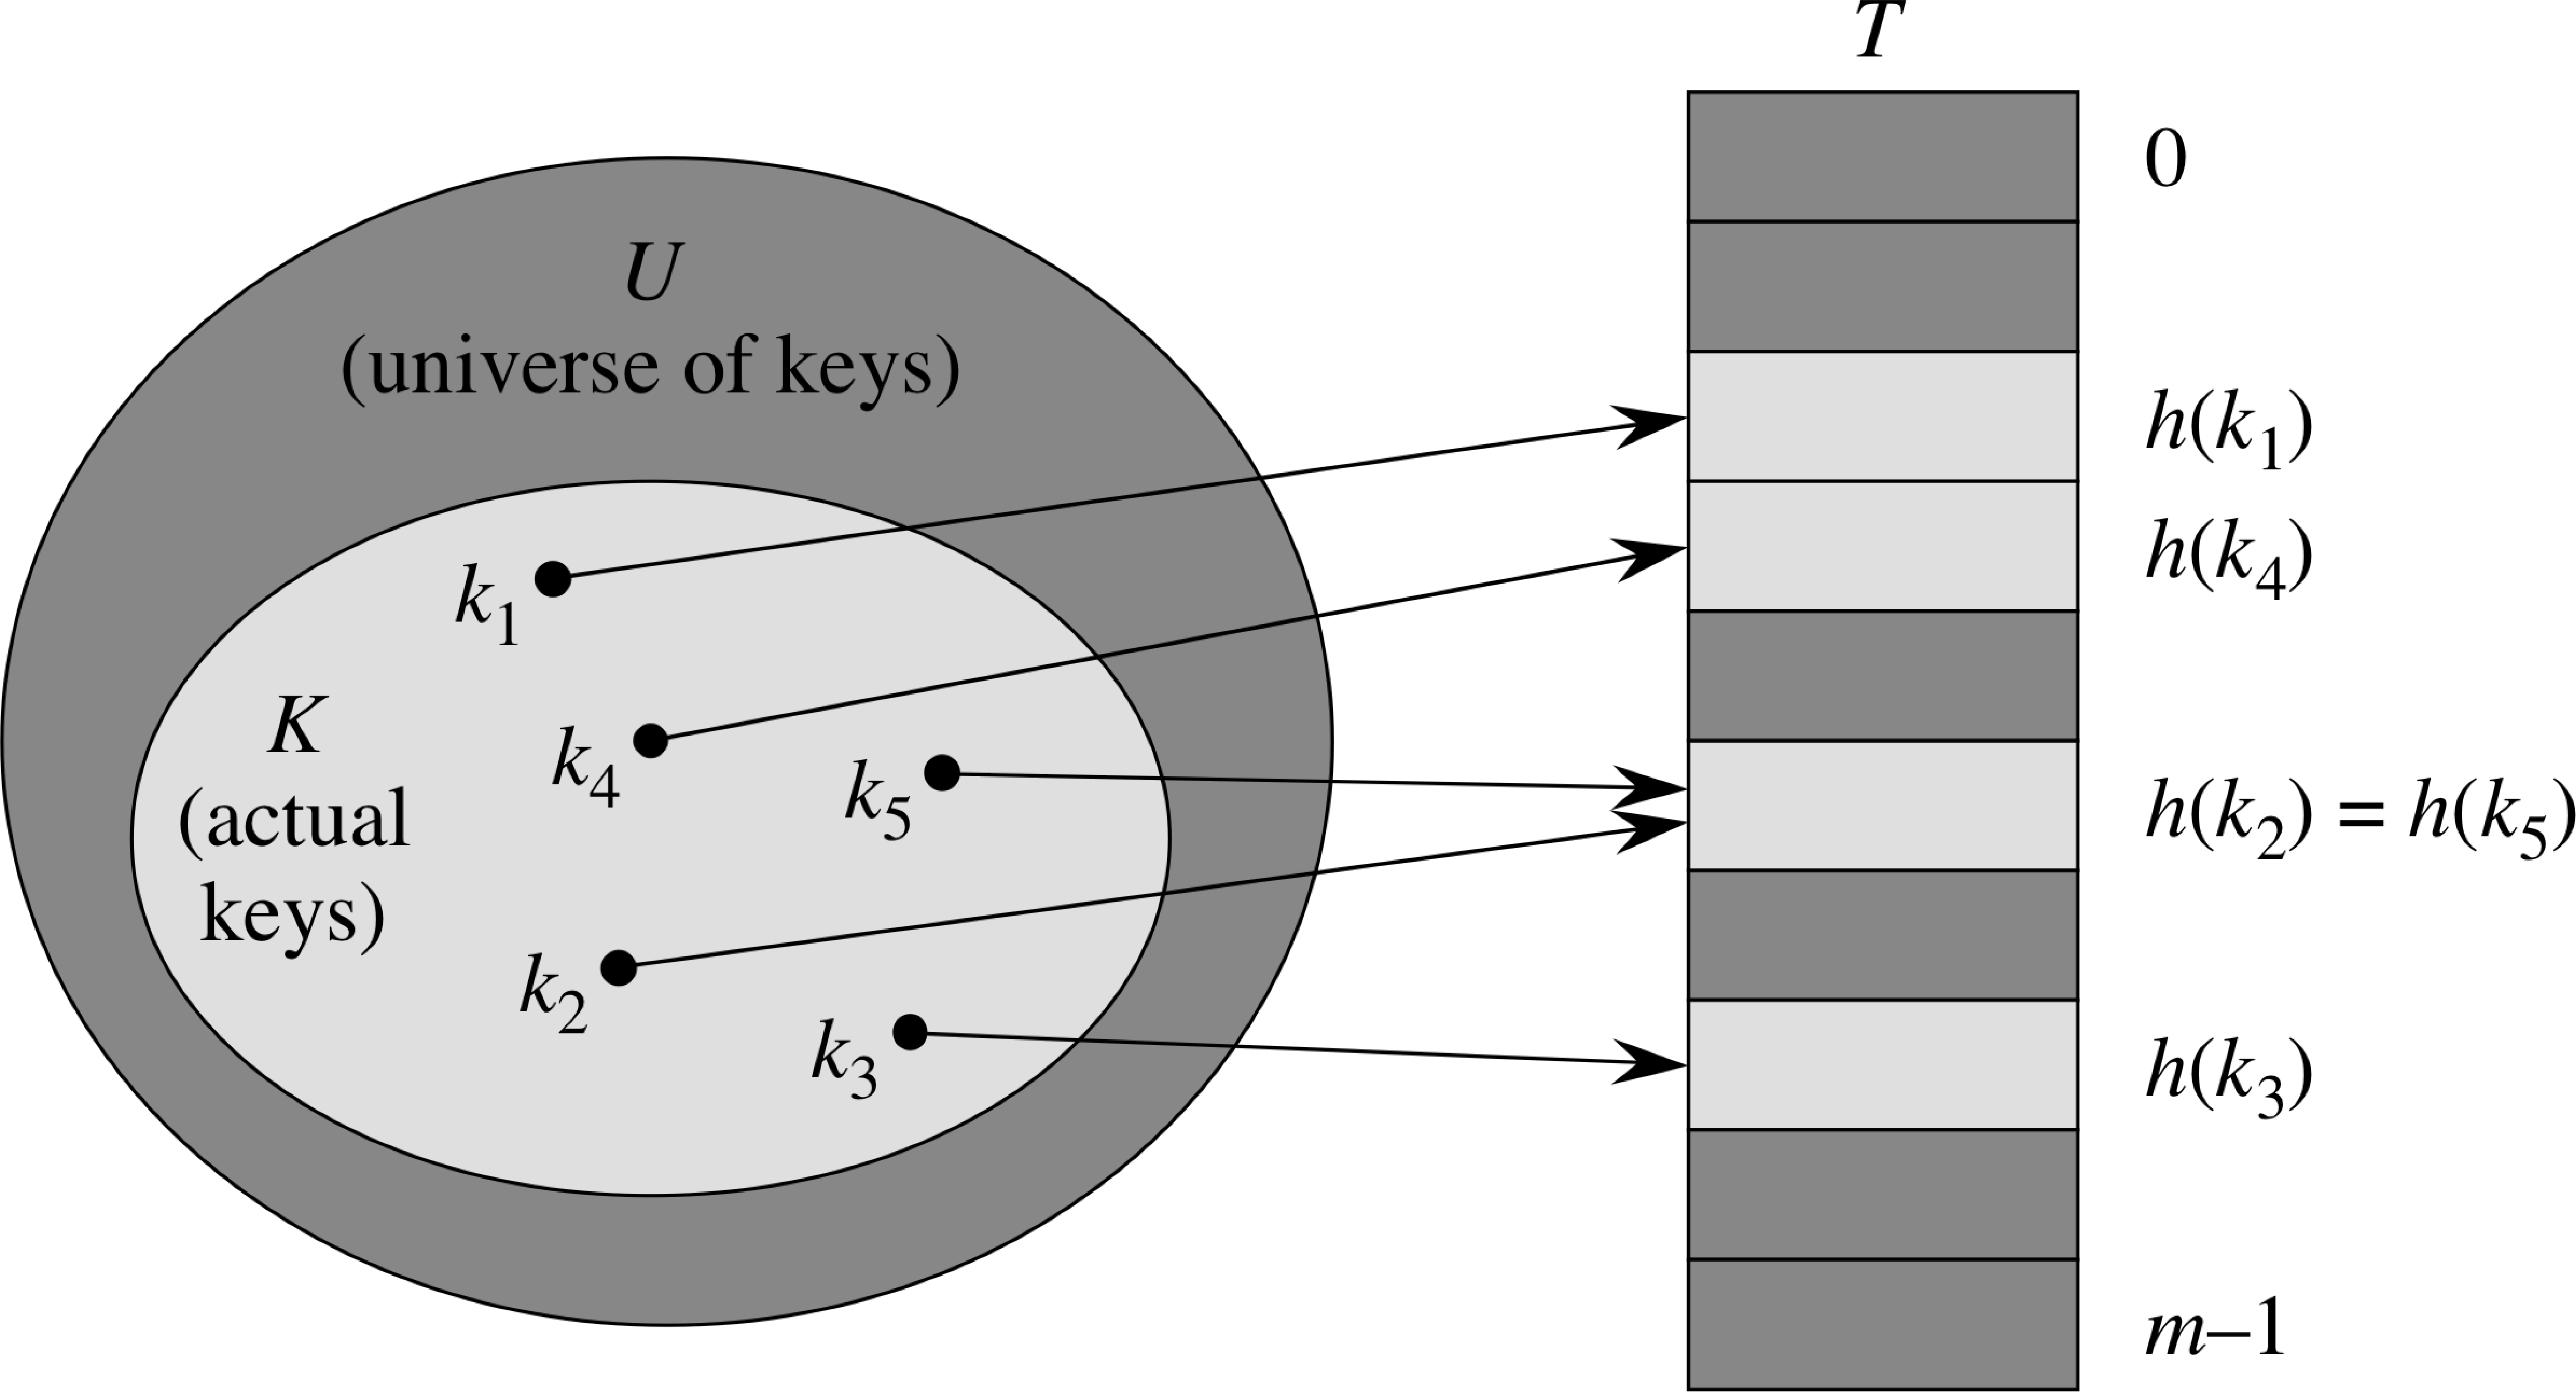
\includegraphics[width=\textwidth]{Fig-11-2.pdf}

\end{frame}

\sect{Collisions}
\bi
\ii When two or more keys hash to the same slot.
\ii Can happen when there are more possible keys than slots ($|U| >
m$).
\ii For a given set $K$ of keys with $|K|\leq m$, may or may not
happen.
\ii Definitely happens when $|K| > m$.
\ii Must be prepared to handle collisions in all cases.
\ii Two methods:
\bi \ii chaining \ii open addressing \ei
\ii Chaining is usually better.

\ei


\end{frame}

\sect{Collision resolution by chaining}
\bi
\ii Put all elements that hash to the same slot into a linked list.
\ei

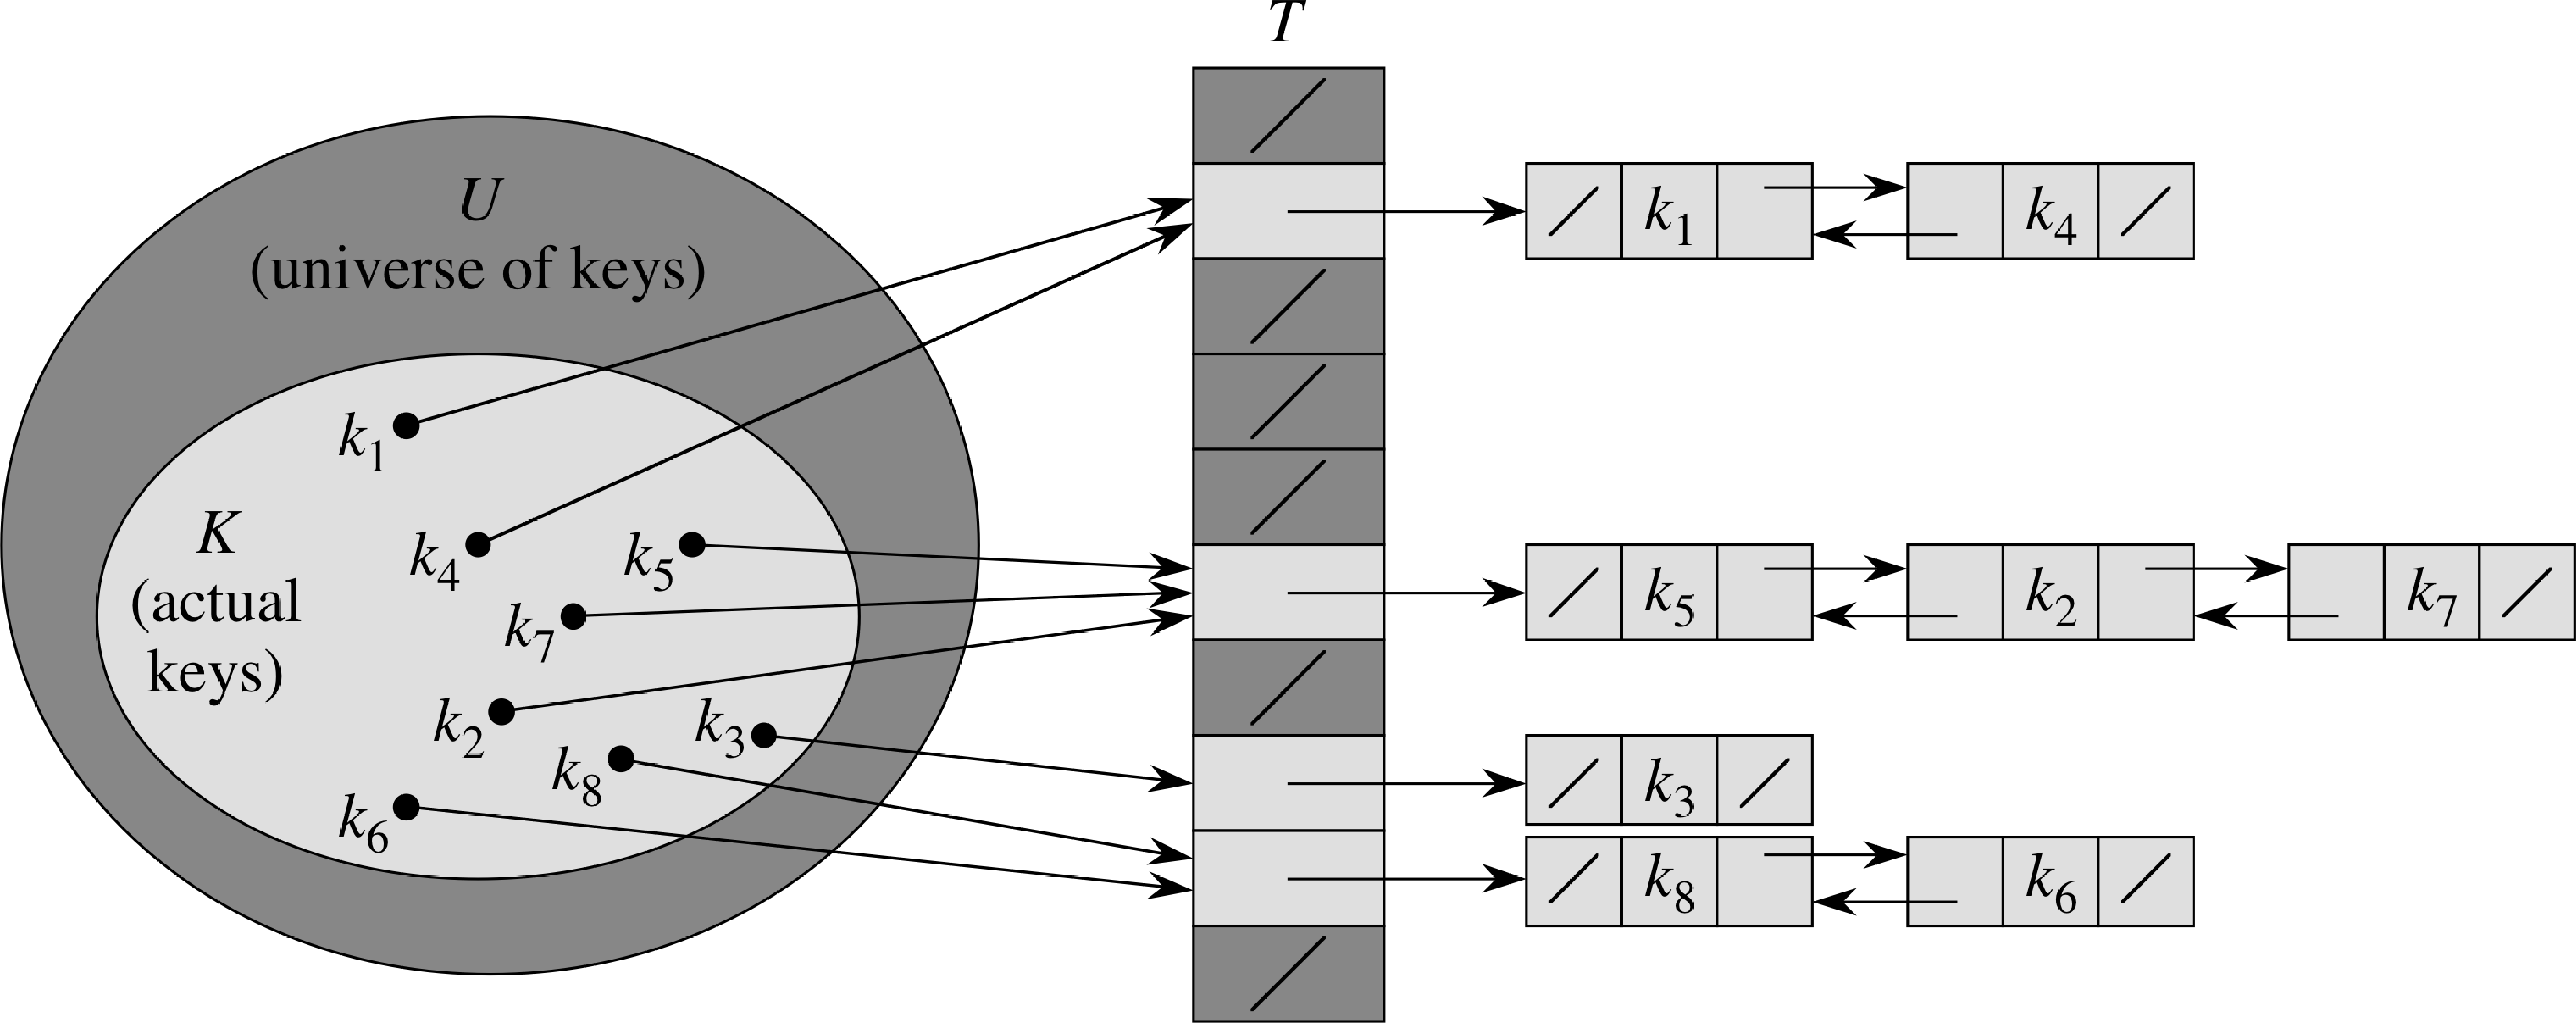
\includegraphics[width=\textwidth]{Fig-11-3.pdf}

\bi
\ii Doubly linked list allows easy deletion.
\ei

\end{frame}

\sect{Implementation of hash table with chaining}

  \begin{codebox}
    \Procname{Chained-Hash-Insert$(T,x)$}
    \li insert $x$ at the head of list $T[h(key[x])]$
  \end{codebox}
  \bi
  \ii Worst case $O(1)$
  \ii Assumes element inserted not already in list.
  \ii Would take an additional search to see if it was already
  inserted.
  \ei

\end{frame}

\sect{Implementation of hash table with chaining}

  \begin{codebox}
    \Procname{Chained-Hash-Search$(T,k)$}
    \li search for element with key $k$ in list $T[h(k)]$
  \end{codebox}
  \bi
  \ii Running time proportional to length of list in slot $h(k)$
  \ei

\end{frame}

\sect{Implementation of hash table with chaining}

  \begin{codebox}
    \Procname{Chained-Hash-Delete$(T,x)$}
    \li delete $x$ from the list $T[h(key[x])]$
  \end{codebox}
  \bi
  \ii Given pointer $x$ to the element to delete, so no search
  is needed to find this element.
  \ii Worst case $O(1)$ if lists are doubly linked.
  \ii If lists are singly linked, deletion takes as long as search,
  because we must find $x$'s predecessor.
  \ei

\end{frame}

\sect{Analysis of hashing with chaining}
\bi
\ii Given a key, how long does it take to find an element with that
key, or determine that there is no element with that key?
\ii Analysis is in terms of the \textbf{load factor} $\alpha = n/m$
\ii $n = $\# elements in the table
\ii $m = $\# slots in the table
\ii Load factor is average number of elements per linked list.
\ii Can have $\alpha < 1$, $\alpha = 1$, or $\alpha > 1$
\ii Worst case is when all $n$ keys hash to the same slot:
\bi
\ii a single list of length $n$
\ii worst case is $\Theta(n)$ plus time to compute $h$
\ei
\ii Average case depends on how well the hash function distributes
keys among slots.
\ei

\end{frame}

\sect{Average-case analysis of hashing with chaining}
\bi
\ii Assume \textbf{simple uniform hashing}: any given element is
equally likely to hash to any of the $m$ slots.
\ii For $j=0,1,\ldots,m-1$, denote the length of the list $T[j]$ by
$n_j$.
\ii $n=n_0+n_1+\cdots+n_{m-1}$
\ii Average value of $n_j$ is $E[n_j] = \alpha = n/m$
\ii Assume we can compute $h$ in $O(1)$ time, so that the time
required to search for $k$ depends on the length $n_{h(k)}$ of the
list $T[h(k)]$.
\ii Two cases:
\bi
\ii Unsuccessful search:  hash table has no element with key $k$
\ii Successful search:  hash table contains an element with key $k$
\ei
\ei

\end{frame}

\sect{Unsuccessful search}

\begin{description}
\item[Theorem] \mbox{}

  An unsuccessful search takes expected time
    $\Theta(1+\alpha)$.

  \item[Proof]\mbox{}
    \bi
    \ii Simple uniform hashing means any key not already in the table
    is equally likely to hash to any of the $m$ slots.
    \ii To search unsuccessfully for any key $k$, need to search to
    the end of the list $T[h(k)]$.
    \ii This list has expected length $\alpha$.
    \ii Adding the time to compute the hash function gives
    $\Theta(1+\alpha)$.
    \ei
\end{description}

\end{frame}

\sect{Successful search}

\bi
\ii The expected time for a successful search is also
$\Theta(1+\alpha)$.
\ii The probability that each list is searched is proportional to the
length of the list.
\ei

\end{frame}

\sect{Successful search}
{\bf Theorem}

  A successful search takes expected time
    $\Theta(1+\alpha)$.

{\bf Proof}
    \bi
    \ii Assume the element $x$ is equally likely to be any of the $n$
    elements stored in the table.
    \ii The number examined during the search for $x$ is 1
    more than the number of elements that appear before $x$ in $x$'s
    list.
    \ii These are the elements inserted {\em after} $x$ was inserted.
    \ii We need to find the average, over $n$ elements, of
    how many elements were inserted into $x$'s list after $x$
    was inserted.
    \ii Let $x_i$ be the $i$th element inserted,
    and let $k_i = key[x_i]$.
    \ii For all $i$ and $j$, let
    $ X_{ij} = I\{h(k_i) = h(k_j)\}$
    \ii Simple uniform hashing means
    \[ Pr\{h(k_k)=h(k_j)\} = 1/m = E[X_{ij}]\]
    \ei


\end{frame}

\sect{Expected number of elements examined, successful search}
\begin{align*}
  E\left[\frac{1}{n}\sum_{i=1}^{n}\left(1+\sum_{j=i+1}^{n}X_{ij}\right)\right]
  &=
  \frac{1}{n}\sum_{i=1}^{n}\left(1+\sum_{j=i+1}^{n}E[X_{ij}]\right)\\
  &=
  \frac{1}{n}\sum_{i=1}^{n}\left(1+\sum_{j=i+1}^{n}\frac{1}{m}\right)\\
  &=
  1+\frac{1}{nm}\sum_{i=1}^{n}(n-i)\\
  &=
  1+\frac{1}{nm}\sum_{i=0}^{n-1}i\\
  &=
  1+\frac{1}{nm}\frac{n(n-1)}{2}\\
  &=
  1+\frac{n-1}{2m}
  = 1 + \frac{\alpha}{2} - \frac{\alpha}{2n} = \Theta(1+\alpha)
\end{align*}

\end{frame}

\sect{Alternative analysis}
\bi
\ii $X_{ij\ell} = {I}\{\mbox{the search is for $x_i$,
  $h(k_i)=h(k_j)=\ell$\}}$
\ii Simple uniform hashing means $Pr\{h(k_i)=\ell\}=Pr\{h(k_j)=\ell\}=
1/m$
\ii $Pr\{\mbox{the search is for $x_i$}\} = 1/n$
\ii All these are independent: $Pr\{X_{ij\ell}=1\} =
{E}[X_{ij\ell}] =1/nm^2 $
\begin{align*}
Y_j &= {I}\{\mbox{$x_j$ appears in a list prior to the
  $x_i$}\}\\
   &= \sum_{i=1}^{j-1}\sum_{\ell=0}^{m-1} X_{ij\ell}
\end{align*}
\ei

\end{frame}

\sect{Alternative analysis, continued}
\begin{align*}
  E\left[1+\sum_{j=1}^n Y_j\right]
  &=
  1 + E\left[\sum_{j=1}^{n}\sum_{i=1}^{j-1}\sum_{\ell=0}^{m-1} X_{ij\ell}\right]\\
  &=
  1 + \sum_{j=1}^{n}\sum_{i=1}^{j-1}\sum_{\ell=0}^{m-1} E[X_{ij\ell}]\\
  &=
  1 + \sum_{j=1}^{n}\sum_{i=1}^{j-1}\sum_{\ell=0}^{m-1} \frac{1}{nm^2}\\
  &=
  1 + {n \choose 2}\cdot m \cdot \frac{1}{nm^2}\\
  &=
  1 + \frac{n-1}{2m}\\
  &=
  1 + \frac{\alpha}{2} - \frac{\alpha}{2n} = \Theta(1 + \alpha)
\end{align*}


\end{frame}

\sect{Interpretation}
\bi
\ii If $n=O(m)$ then $\alpha = n/m = O(1)$, which means searching
takes constant time on average.
\ii Since insertion  and deletion take $O(1)$ worst case time,
all dictionary operations take average time $O(1)$.
\ei

\end{frame}

\sect{Hash functions}
\bi
\ii Ideally, satisfies the assumption of simple uniform hashing.
\ii In practice, impossible since we don't know the
distribution of input keys.
\ii Often use heuristics, based on the domain of the keys,
to create hash functions that work well.
\ei

\end{frame}

\sect{Keys as natural numbers}
\bi
\ii Hash functions usually assume keys are natural numbers.
\ii Can interpret any computer data as natural number.
\ii Interpret as radix $2^p$ number.
\ii Strings, for example: \textsc{CLRS}
\bi
\ii ASCII: 67, 76, 82, 83
\ii There are 128 ASCII values, use radix $2^7$:
\ii $h(\textsc{CLRS}) = 67(128^3) + 76(128^2) + 82(128^1) + 83(128^0) = 141,764,947$
\ei
\ei

\end{frame}

\sect{Division method for hash functions}
\[ h(k) = k \mbox{ mod } m \]
\bi
\ii Example:  $m=20$ and $k=91 \Rightarrow h(k) = 11$
\ii Fast: requires only one division.
\ii Bad ideas:
\bi
\ii Powers of 2 are bad values for $m$:\\ just uses least significant bits.
\ii If $k$ is a character string interpreted as radix $2^p$ number,
then $m=2^p-1$ is bad:  permuting characters does not change hash value.
\ei
\ii Good choice for $m$:\\  Prime number not too close to a power of 2.
\ei
\end{frame}

\sect{Division method example}
\bi
\ii Store $n \approx 2000$ character strings.
\ii Don't mind searching 3 strings per unsuccessful search.
\ii Choose $m=701$.
\ii This is a prime near $2000/3$ but not near any power of 2.
\ei


\end{frame}

\sect{Multiplication method for hash functions}

  \begin{enumerate}
  \ii Choose $0 < A < 1$
  \ii Multiply $k$ by $A$
  \ii Extract the fractional part
  \ii Multiply by $m$
  \ii Take the floor.
  \end{enumerate}

\begin{align*}
  h(k) &= \lfloor m (kA \mbox{ mod } 1)\rfloor
\end{align*}
where
\[
kA\mod 1 = kA-\lfloor kA\rfloor
\]
gives the fractional part.

\end{frame}

\sect{Easy implementation of: $  h(k) = \lfloor m (kA \mbox{ mod } 1)\rfloor$}
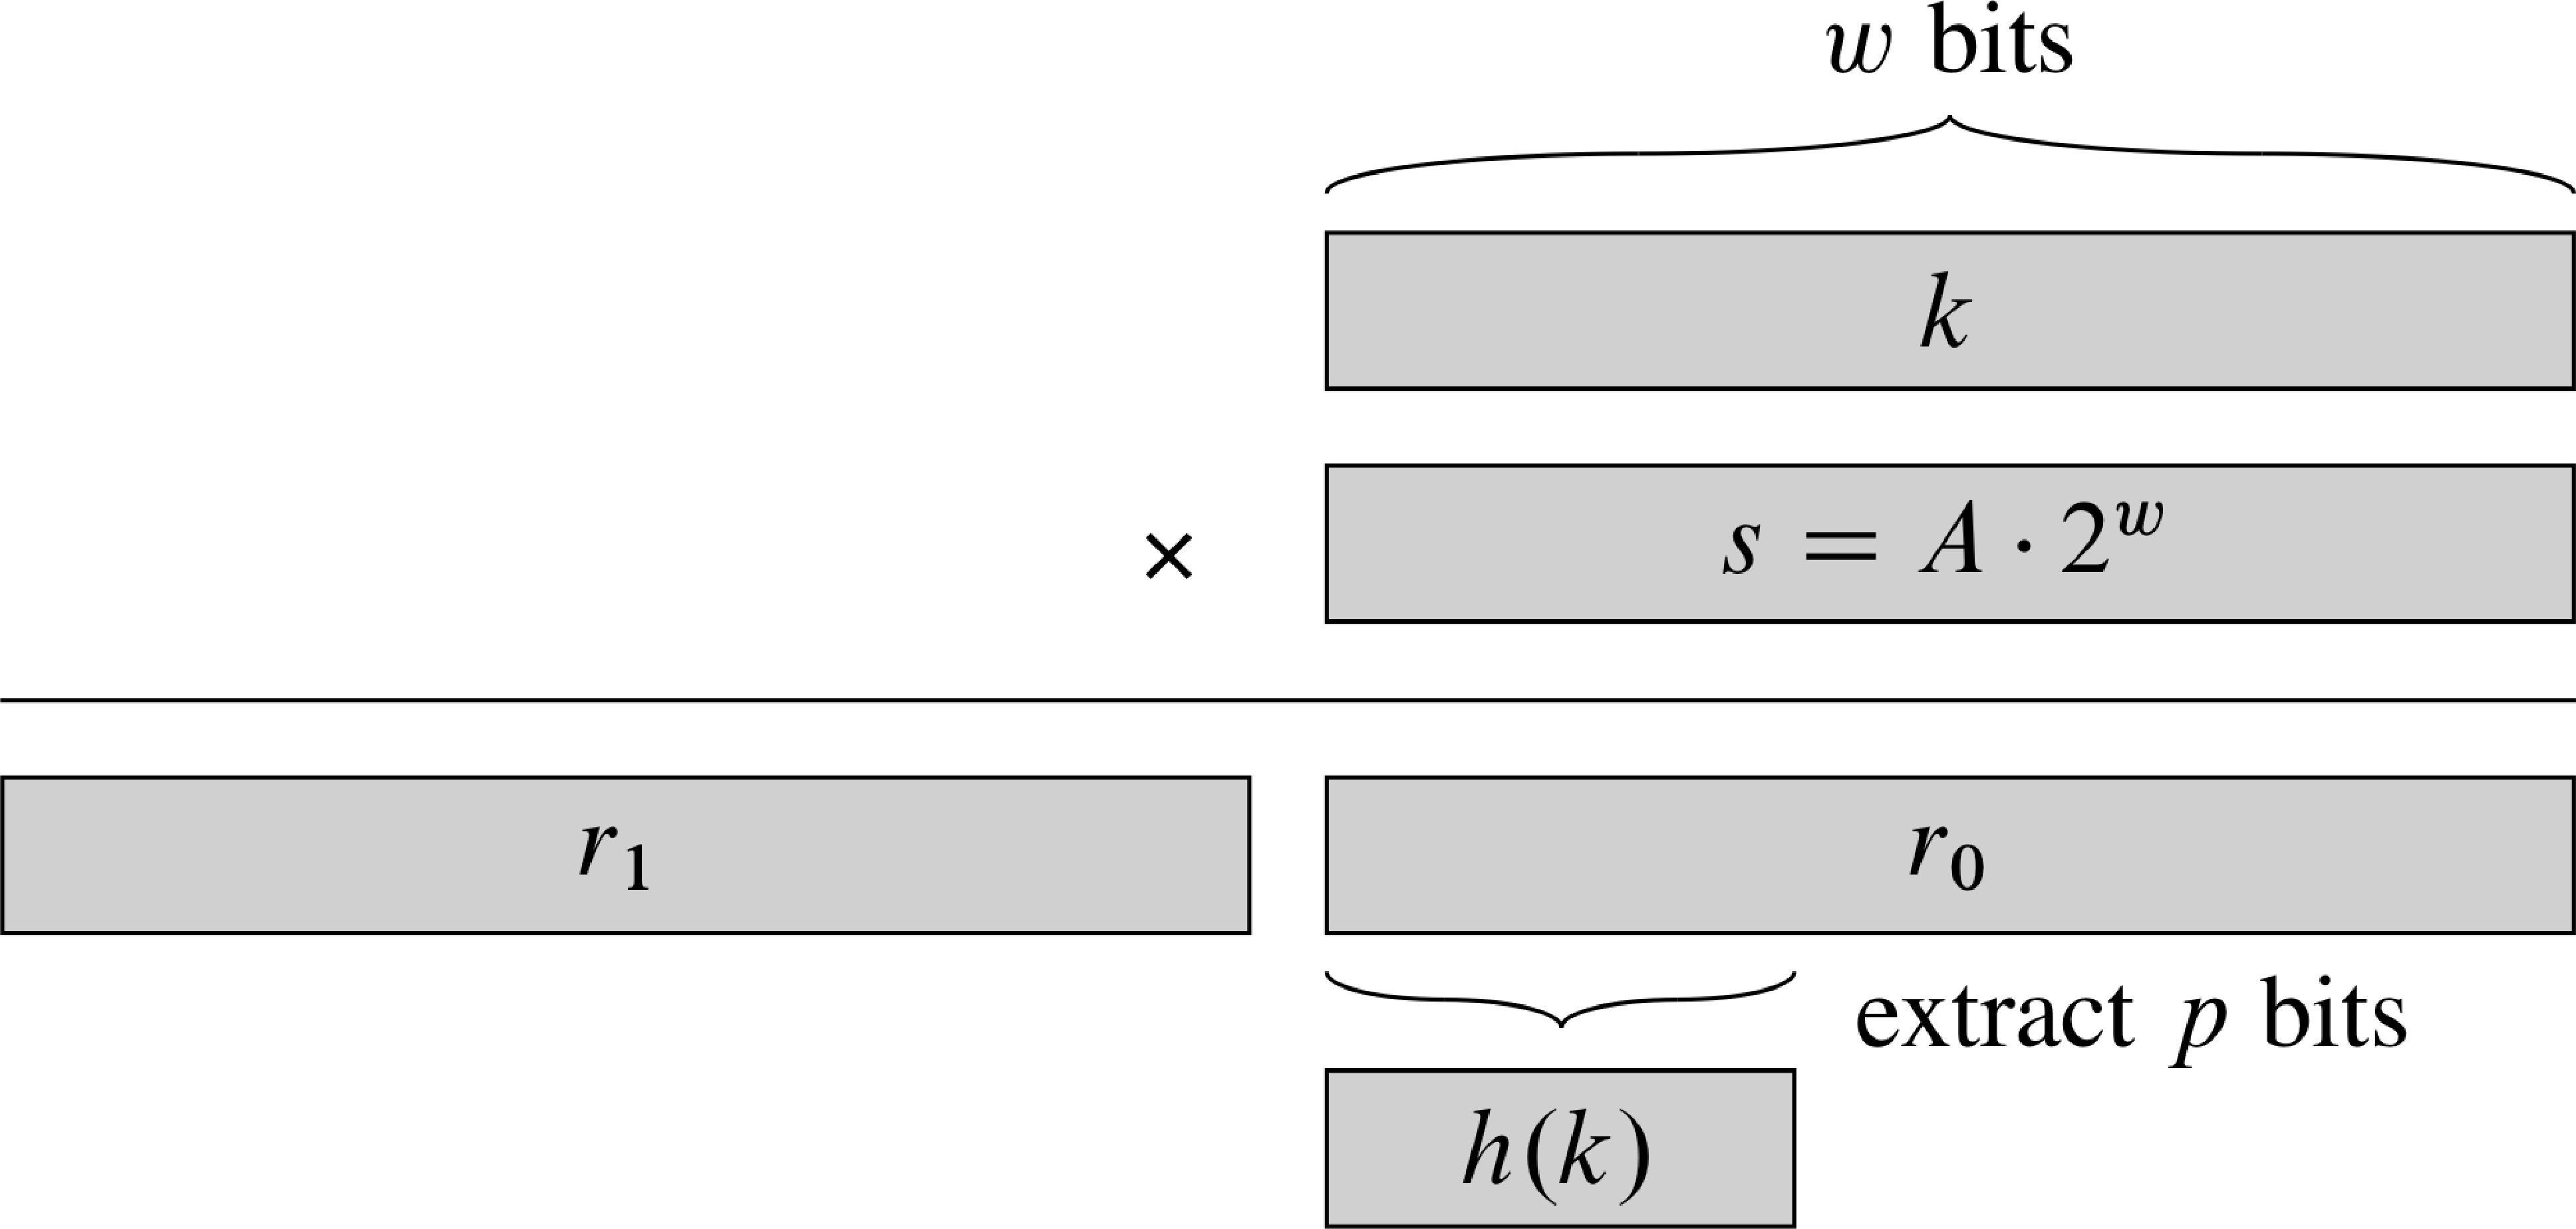
\includegraphics[scale=0.12]{Fig-11-4.pdf}

\bi
\ii Choose $m=2^p$.
\ii Let word size be $w$ bits.
\ii Assume $k$ fits in a single word.
\ii Let $s$ be an integer in the range $0<s<2^w$.
\ii Let $A$ be $s/2^w$.
\ei
\end{frame}

\sect{Easy implementation of: $  h(k) = \lfloor m (kA \mbox{ mod } 1)\rfloor$}
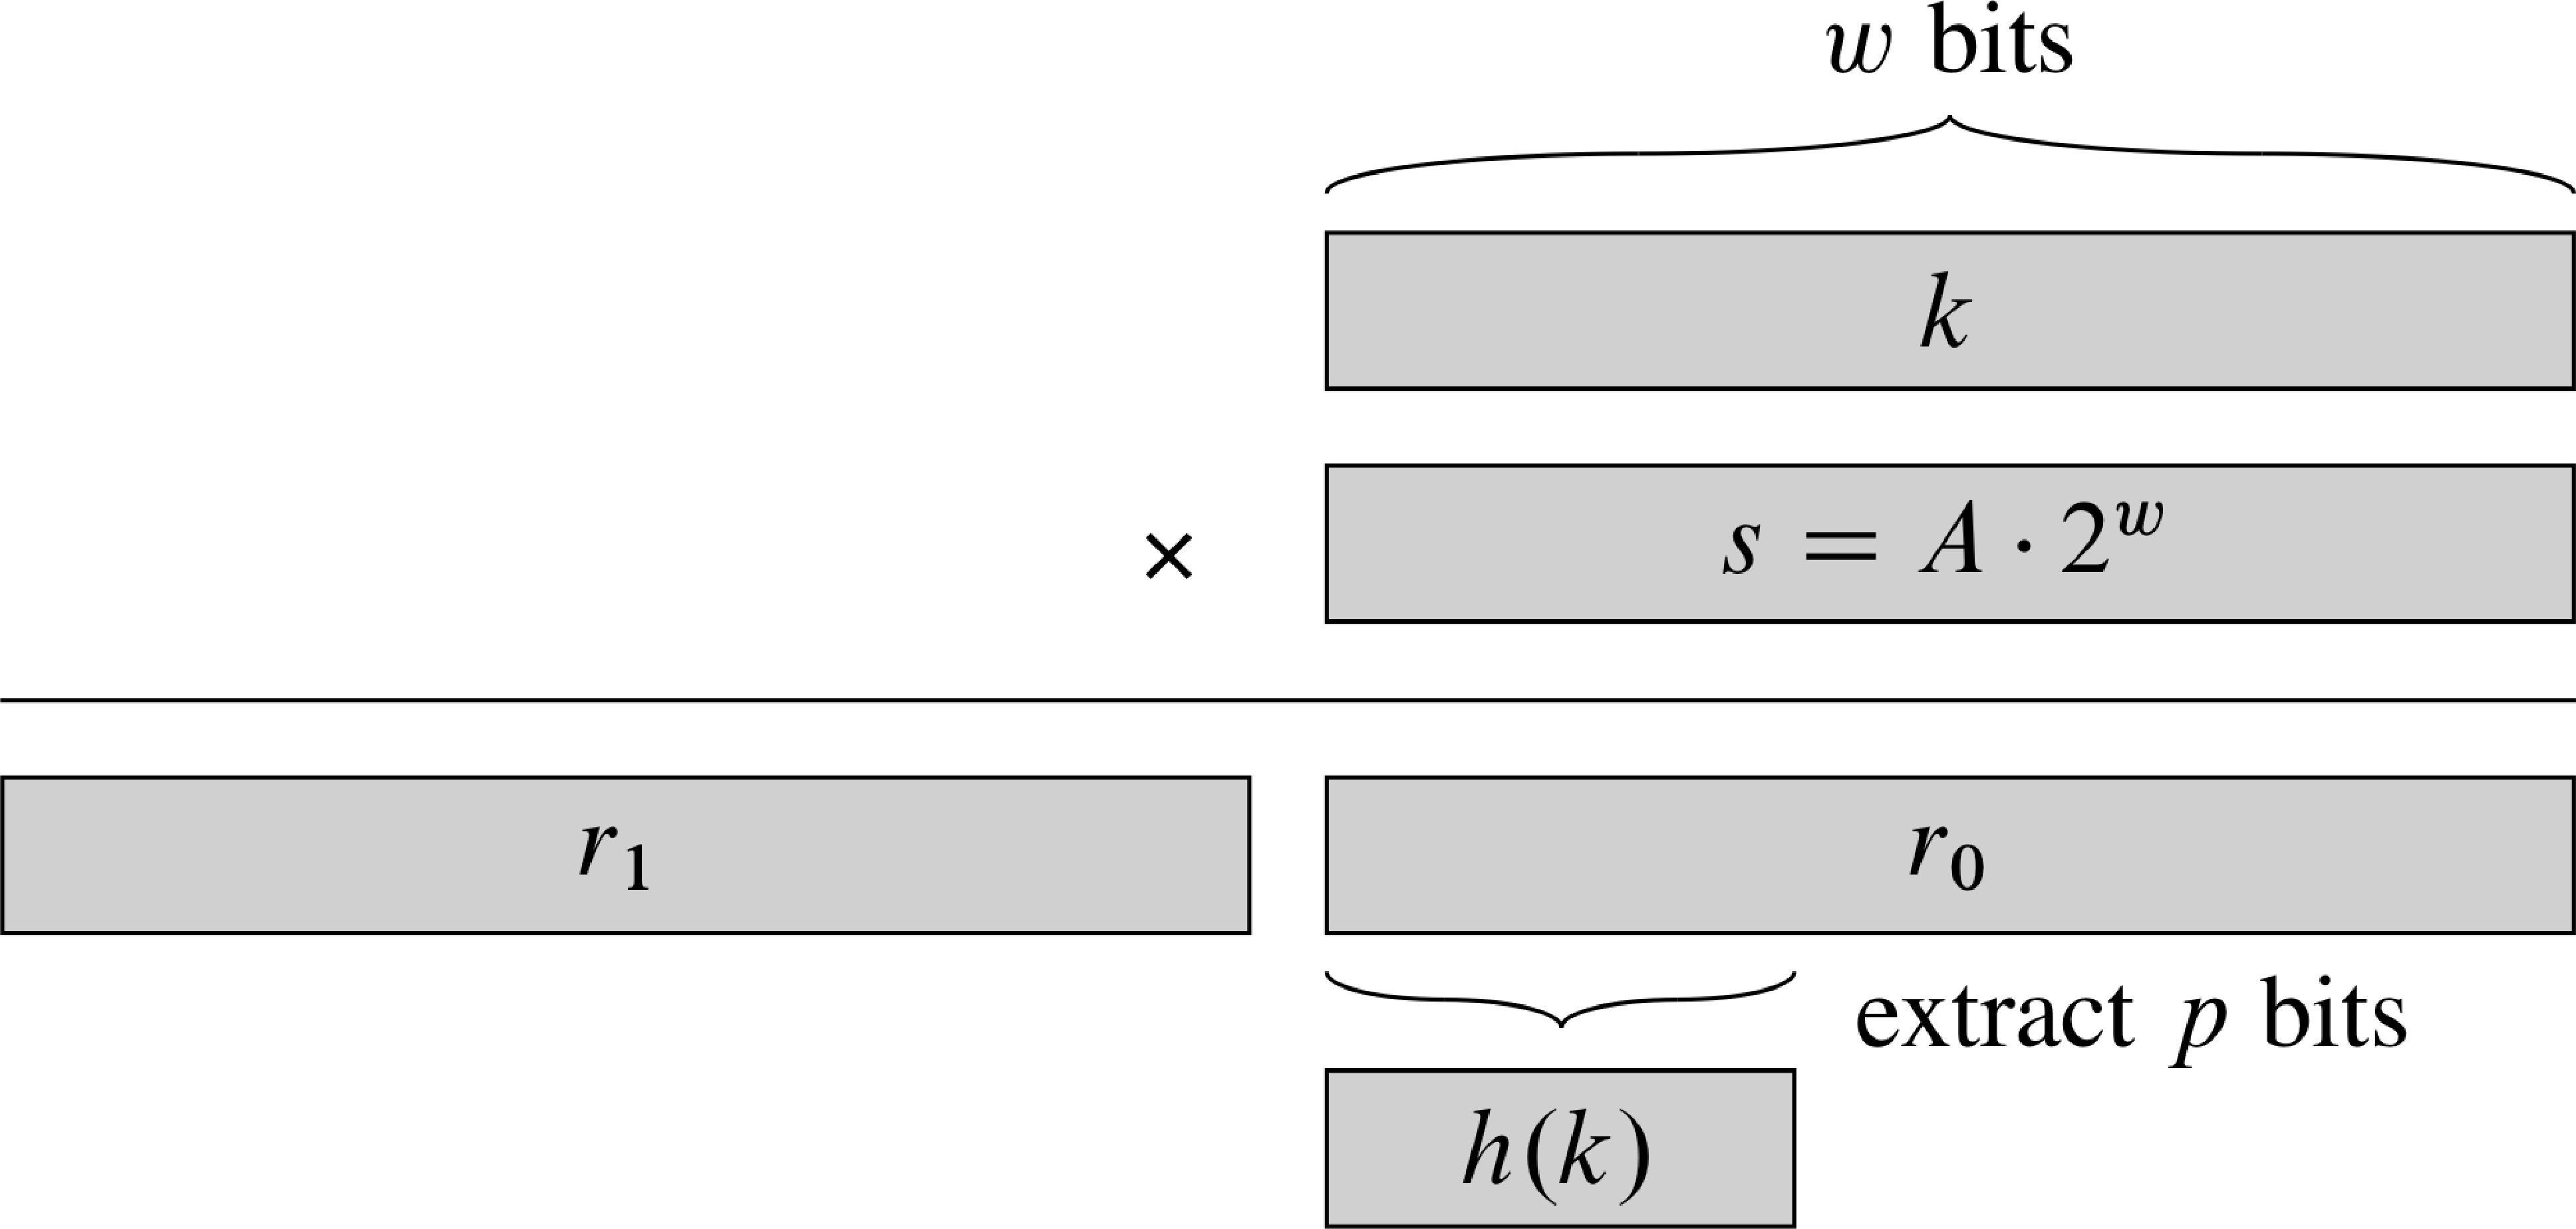
\includegraphics[scale=0.12]{Fig-11-4.pdf}

\bi
\ii Multiply $k$ by $s$.
\ii Result is $2w$ bits.
\ii We can ignore $r_1$, since $r_0$ is the fractional part.
\ii Multiplying by $m=2^p$ just shifts $r_0$ left $p$ places.
\ii Instead, just take the $p$ most significant bits of $r_0$.
\ei
\end{frame}

\sect{Example computation of: $  h(k) = \lfloor m (kA \mbox{ mod } 1)\rfloor$}

\bi
\ii Choose $m=2^3=8$, $w=5$, $k=21$.
\ii Choose $0 < s < 2^5$, s = 13, therefore $A = 13/32$.
\ei
\hrulefill
\bi
\ii $kA = 21(13/32) = 273/32 = 8\frac{17}{32}$
\ii $kA\mod 1 = 17/32$
\ii $m(kA\mod 1) = 8(17/32) = 17/4 = 4\frac{1}{4}$
\ii $\lfloor m(kA\mod 1)\rfloor = 4 = h(k)$
\ei
\hrulefill
\begin{multicols}{2}
  \bi
  \ii $ks = 21(13) = 273 = 8(2^5) + 17$
  \ii $r_1 = 8$, $r_0=17 = 10001_b$.
  \ii $p=3$ most significant bits is $100_b = 4$.
  
  \ei
\columnbreak
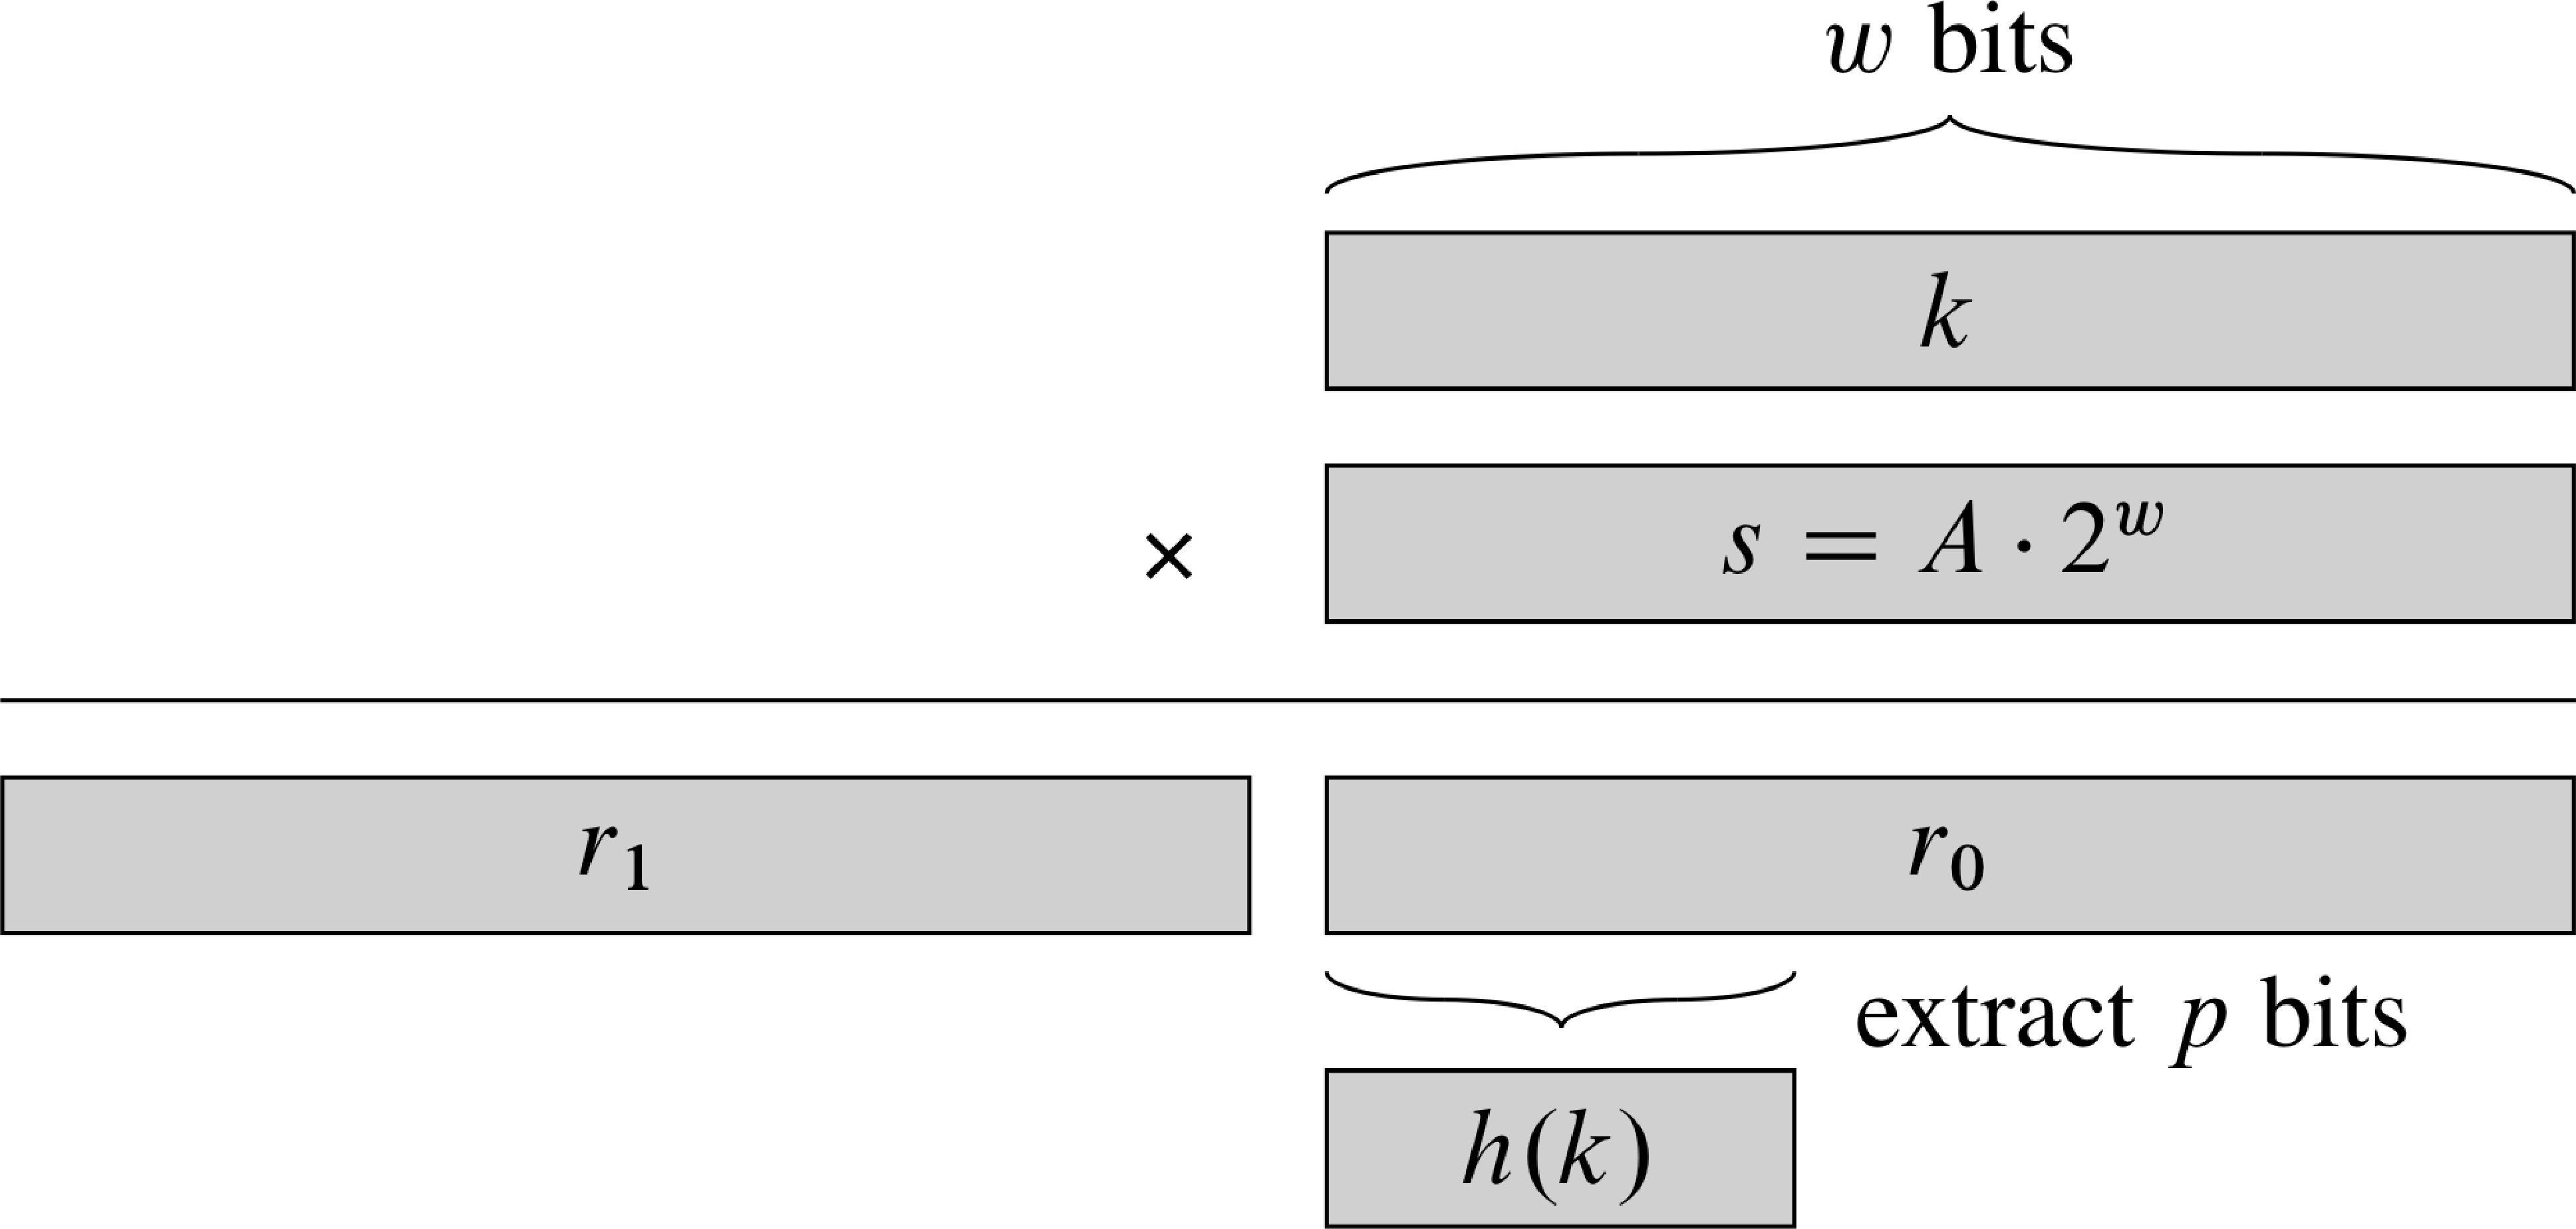
\includegraphics[scale=0.08]{Fig-11-4.pdf}
\end{multicols}

\end{frame}


\sect{Multiplication method for hash functions}
  \[h(k) = \lfloor m ((kA) \mbox{ mod } 1)\rfloor\]
\bi
\ii Disadvantage: slower than division method.
\ii Advantage: value of $m$ is not critical, $2^p$ a good choice.
\ii Knuth suggests a value for $A$:
\[\frac{\sqrt{5} -1}{2} = 0.6180339887... \]
\ii  Look up the Golden Ratio.
\ei
\hfill\tikz[overlay]\node{\makebox{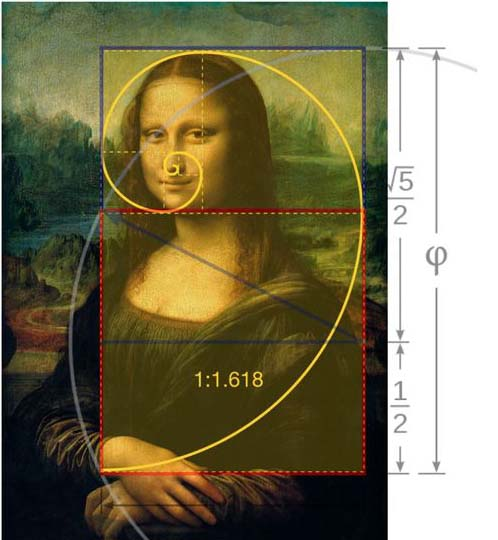
\includegraphics[scale=0.25]{monalisa}}};
\vfill
\end{frame}


\sect{Universal hashing---randomized hashing}
\bi
\ii For any hash function, the world {\em could} give us
keys that all hash to the same spot.  If the world was very, very mean.

\ii To randomize this, choose a hash function randomly from a
collection of hash functions, each time the program starts.

\ii A collection of hash functions, $\mathcal{H}$ that map a universe
$U$ into keys $0\leq k < m$ is called {\bf universal} if
for each pair, $k,\ell\in U$, $k\neq \ell$, 
\[
\mbox{Pr}_{h\in \mathcal{H}} \{h(k) = h(\ell)\} \leq \frac{1}{m}
\]

\ii In other words, the chance of a collision between $k$ and $\ell$
is no more than $1/m$, when $h$ is chosen at random from $\mathcal{H}$.
\ii Such collections of hash functions are easy to design.

\ei
\end{frame}
\sect{Universal hashing expected chain lengths}
Using chaining and universal hashing on key $k$:
\bi
\ii If $k$ is not in the table,
\[ E[n_{h(k)}] \leq \alpha \]
\ii If $k$ is in the table,
\[ E[n_{h(k)}] \leq 1 + \alpha \]
\ii
So the expected time for {\sc Search} is $O(1)$.
\ei
\end{frame}



\sect{Open addressing}

\bi
\ii Instead of chaining, store all keys in hash table.
\ii Must have $\alpha \leq 1$.
\ii Use $h(key)+i\mod m, i=0,1,2,...m-1$ 
\ii Example:  $h(n) = n\mod 10$ 
\ei
\vfill

\begin{tabular}{|r|c|c|c|c|c|c|c|c|c|c|}\hline
Index:&  0&1&2&3&4&5&6&7&8&9\\\hline
Insert 12: & {\sf x} &{\sf x} &12 &{\sf x} &{\sf x} &{\sf x} &{\sf x} &{\sf x} &{\sf x} &{\sf x} \\\hline
Insert 14:& {\sf x} &{\sf x} &12 &{\sf x} &14 &{\sf x} &{\sf x} &{\sf x} &{\sf x} &{\sf x} \\\hline
 Insert 32:& {\sf x} &{\sf x} &12 &32 &14 &{\sf x} &{\sf x} &{\sf x} &{\sf x} &{\sf x} \\\hline
 Insert 92:& {\sf x} &{\sf x} &12 &32 &14 &92 &{\sf x} &{\sf x} &{\sf x} &{\sf x} \\\hline
 Insert 53: & {\sf x} &{\sf x} &12 &32 &14 &92 &53 &{\sf x} &{\sf x} &{\sf x} \\\hline
  \end{tabular}

\vfill

\bi
\ii Linear probing like this leads to \textbf{clustering}.
\ei
\end{frame}

\sect{Open addressing}
\bi
\ii More generally, use a hash function that takes both a key and a
position and returns a position:
\[
h : U\times \{0,1,...,m-1\} \rightarrow \{0,1,...,m-1\}
\]
\ii
Then use probe sequence
\[
h(k,0), h(k,1), ..., h(k,m-1)
\]
\ii
We require that for every key, $k$, the probe sequence
be a permutation of
\[
(0, 1, ..., m-1)
\]
so that all possible probes are examined in $m$ probes.
\ii
Linear probing satisfies this requirement, but has bad clustering.
\ei

\end{frame}

\sect{Hash insertion and search, open addressing}
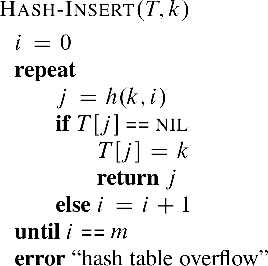
\includegraphics{Hash-Insert}
\hfill
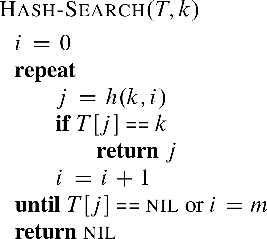
\includegraphics{Hash-Search}
\end{frame}

\sect{Hash deletion, open addressing}

\bi
\item We cannot simply replace a deleted element with {\sc nil}.
\item
  This might make search halt prematurely if clustering has occurred.
\item
  Instead we insert a special {\sc deleted} value.
\item
  Insert will treat {\sc deleted} as available.
\item
  Search will treat {\sc deleted} as full.
\item
  Search time no longer depends on $\alpha$ alone.
\ei
\end{frame}

\sect{Uniform hashing with open addressing}
\bi
\ii
In our analysis, we assume {\bf uniform hashing}:
\bi\ii
The probe sequence for a key $k$
is equally likely to be any of the $m!$ possible
sequences.\ei
\ii
Open addressing has to generalize the notion of
uniform hashing to a function that generates an entire sequence of
probes.
\ii True open uniform hashing is difficult.
\ii In practice approximations are used.
\ei
\end{frame}


\sect{Linear probing}
\bi
\ii
Given an ordinary hash function $h' : U \rightarrow \{0,...,m-1\}$,
called an {\bf auxiliary hash function}, use
\[
h(k,i) = (h'(k) + i) \mod m
\]
\ii
Only generates $m$ of the $m!$ possible permutations of $\{0,...,m-1\}$
\ii
Extremely susceptible to {\bf primary clustering}.
\ii
Any slot preceded by $i$ full slots gets filled with probability
\[\frac{i+1}{m}\]
and hence long chains get longer.
\pause
\ii
Note: it does not matter if we use \[h(k,i) = h'(k) + ai + b\].  Why not?
\ei
\end{frame}

\sect{Quadratic probing}

\[
h(k,i) = (h'(k) + c_1i + c_2i^2)\mod m
\]
\bi
\ii $c_1, c_2, m$ must be carefully selected.
\ii
Primary clustering is eliminated.
\ii
If two keys have the same initial probe, their entire sequence
is the same.
\ii
This is called {\bf secondary clustering} and is not as serious.
\ii
Only $m$ of the $m!$ possible permutations of $\{0,...,m-1\}$ are
used. 
\ei
\end{frame}

\sect{Double hashing}
\[
h(k,i) = (h_1(k) + i h_2(k)) \mod m
\]
\bi
\ii Needs two auxiliary hash functions, $h_1, h_2$.
\ii $h_2(k)$ must be relatively prime to $m$:
\bi
\ii Let $m=2^p$ and make $h_2(k)$ odd.
\ii Let $m$ be prime and make $h_2(k) < m$:
\begin{align*}
  h_1(k) &= k \mod m\\
  h_2(k) &= 1 + (k \mod (m-1))
\end{align*}
\ei
\ii $\Theta(m^2)$ probe sequences used, instead of $\Theta(m)$.
\ii Performance is very close to ideal uniform hashing.
\ei
\end{frame}


\sect{Double hashing}
\begin{multicols}{2}
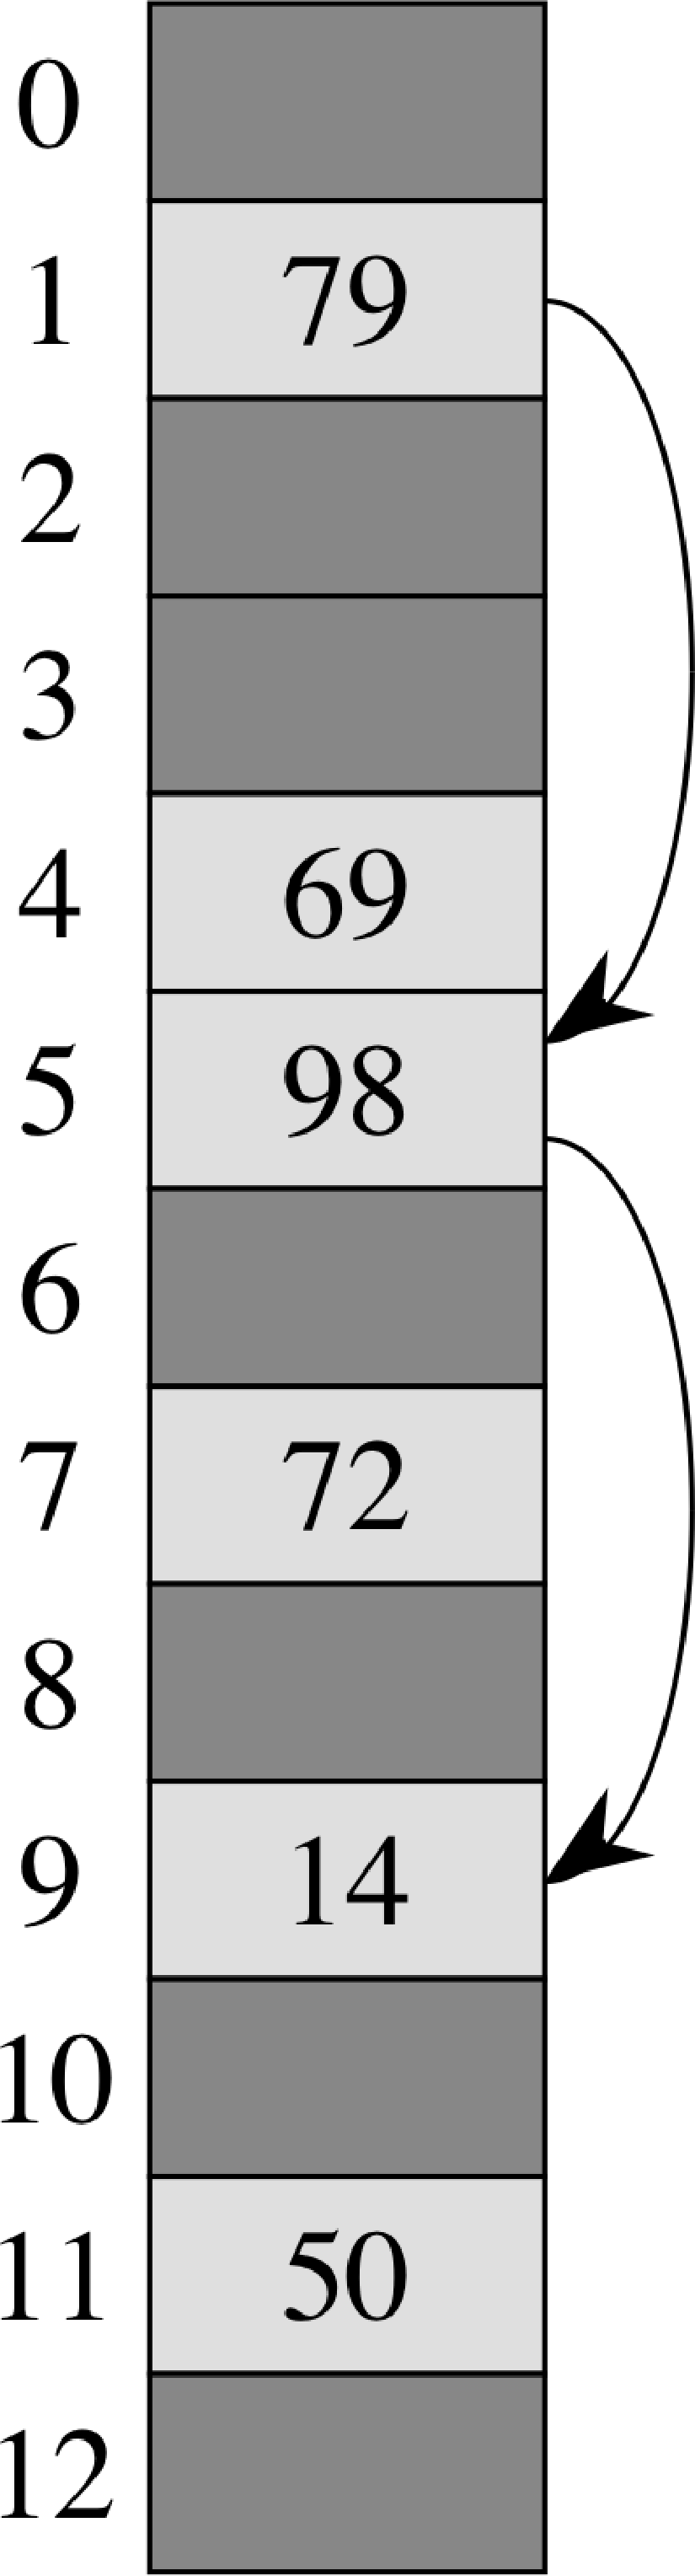
\includegraphics[height=0.75\textheight]{Fig-11-5.pdf}
\columnbreak
\begin{align*}
  h_1(k) &= k \mod 13\\
  h_2(k) &= 1 + (k \mod 11)\\\\
  h_1(14) &= 1\\
  h_2(14) &= 4
\end{align*}

\end{multicols}
\end{frame}

\sect{Analysis of open-address hashing, unsuccessful search}

{\bf Theorem 11.6}

Assuming uniform hashing
and an open-address hash table with load factor
$
\alpha = {n}/{m} < 1
$
the expected number of probes in an unsuccessful search is at most
$
{1}/{(1-\alpha)}
$.

{\bf Proof}

\begin{align*}
  X &= \mbox{number of probes in unsuccessful search}\\
  A_k &= \{\mbox{$k$th probe is to an occupied slot}\}\\
\{X\geq i\} &= \bigcap_{k=1}^{i-1} A_k\\
\pr{X\geq i} &=
\pr{A_1}\cdot\pr{A_2|A_1}\cdot\pr{A_3|A_1\cap A_2}\\&\cdots
\\&\cdot\pr{A_{i-1}|A_1\cap A_2\cap ...\cap A_{i-2}}
\end{align*}
\end{frame}

\sect{Probability that $i$ probes find occupied slot}
\begin{align*}
  X &= \mbox{number of probes in unsuccessful search}\\
  A_k &= \{\mbox{$k$th probe is to an occupied slot}\}\\
\{X\geq i\} &= \bigcap_{k=1}^{i-1} A_k\\
\pr{X\geq i} &=
\pr{A_1}\cdot\pr{A_2|A_1}\cdot\pr{A_3|A_1\cap A_2}\\&\cdots
\\&\cdot\pr{A_{i-1}|A_1\cap A_2\cap ...\cap A_{i-2}}\\
&= \frac{n}{m}\cdot\frac{n-1}{m-1}\cdot\frac{n-2}{m-2}\cdots
\frac{n-i+2}{m-i+2} \\
&\leq \left(\frac{n}{m}\right)^{i-1}\\
&= \alpha^{i-1}
\end{align*}
\end{frame}


\sect{Expected number of probes in unsuccessful search}
\begin{align*}
  E[X] &= \sum_{i=1}^\infty \pr{X\geq i}\\
  &\leq \sum_{i=1}^\infty \alpha^{i-1}\\
  &= \sum_{i=0}^\infty \alpha^{i}\\
  &= \frac{1}{1-\alpha}\\
  &= 1 + \alpha + \alpha^2 + \alpha^3 + \alpha^4 + \cdots
\end{align*}
\vfill
\bi
\ii The last expression gives us an intuitive picture.
\ei

\end{frame}


\sect{Analysis of open-address hashing, unsuccessful search}

{\bf Theorem 11.6}

Assuming uniform hashing
and an open-address hash table with load factor
$
\alpha = {n}/{m} < 1
$
the expected number of probes in an unsuccessful search is at most
$
{1}/{(1-\alpha)}
$.

\bi
\ii If $\alpha = 0.5$, then we expect less than 2 probes on average. 
\ii If $\alpha = 0.9$, then we expect less than 10 probes on average.
\ei
\end{frame}

\sect{Expected number of probes for {\sc Hash-Insert}}

\bi
\ii An element is inserted after finding an open slot.
\ii This is the same procedure followed by an unsuccessful search.
\ii Therefore the expected number of probes is at most
\[\frac{1}{1-\alpha}\]
\ei

\end{frame}

\sect{Analysis of open address hashing, successful search}

{\bf Theorem 11.8}

Assuming uniform hashing and every key is equally likely,
in an open-address hash table with load factor $\alpha < 1$
the expected number of probes in a successful search is at most
\[
\frac{1}{\alpha}\ln\frac{1}{1-\alpha}
\]

{\bf Proof}

\bi
\ii A successful search does the same as when the $k$ was
inserted.
\ii If $k$ was the $i$th key inserted, then $\alpha = i/m$ when
inserted.
\ii Therefore there were at most $1/(1-i/m) = m/(m-i)$ probes
\ii The average over all $n$ keys is then
\[  \frac{1}{n}\sum_{i=0}^{n-1}\frac{m}{m-i}\]
\ei
\end{frame}


\sect{Averaging over the $n$ keys in the table:}

\begin{align*}
  \frac{1}{n}\sum_{i=0}^{n-1}\frac{m}{m-i}
  &= \frac{m}{n}\sum_{i=0}^{n-1}\frac{1}{m-i}\\
  &= \frac{1}{\alpha} \sum_{k=m-n+1}^m \frac{1}{k}\\
  &\leq \frac{1}{\alpha}\int_{m-n}^m (1/x)dx\\
  &= \frac{1}{\alpha}\ln \frac{m}{m-n}\\
  &= \frac{1}{\alpha}\ln \frac{1}{1-\alpha}\\
\end{align*}
\end{frame}


\sect{Analysis of open address hashing, successful search}

{\bf Theorem 11.8}

Assuming uniform hashing and every key is equally likely,
in an open-address hash table with load factor $\alpha < 1$
the expected number of probes in a successful search is at most
\[
\frac{1}{\alpha}\ln\frac{1}{1-\alpha}
\]

\bi
\ii If $\alpha = 0.5$, then we expect less than 1.387 probes on
average.
\ii If $\alpha = 0.9$, then we expect less than 2.559 probes on
average. 
\ei

\end{frame}

\sect{Perfect hashing}

\bi
\ii In some applications the keys are static:
\bi
\ii Reserved words in a programming language.
\ii File names on a write-only CD-rom.
\ei
\ii In this case we can guarantee {\bf worst-case} $O(1)$.
\ii Use a double hashing scheme.
\ii Choose a good primary $h$ from a universal hash, $\mathcal{H}$.
\ii For each slot $j$, choose a $h_j$ into a secondary hash table, $S_j$.
\ii If size of $S_j$ is proportional to $n_j^2$, we can find
$h_j$ with no collisions.
\ii If we choose $h$ carefully, expected
size of all secondary hash tables is
still $O(n)$.
\ei

\end{frame}

\sect{Perfect hashing}
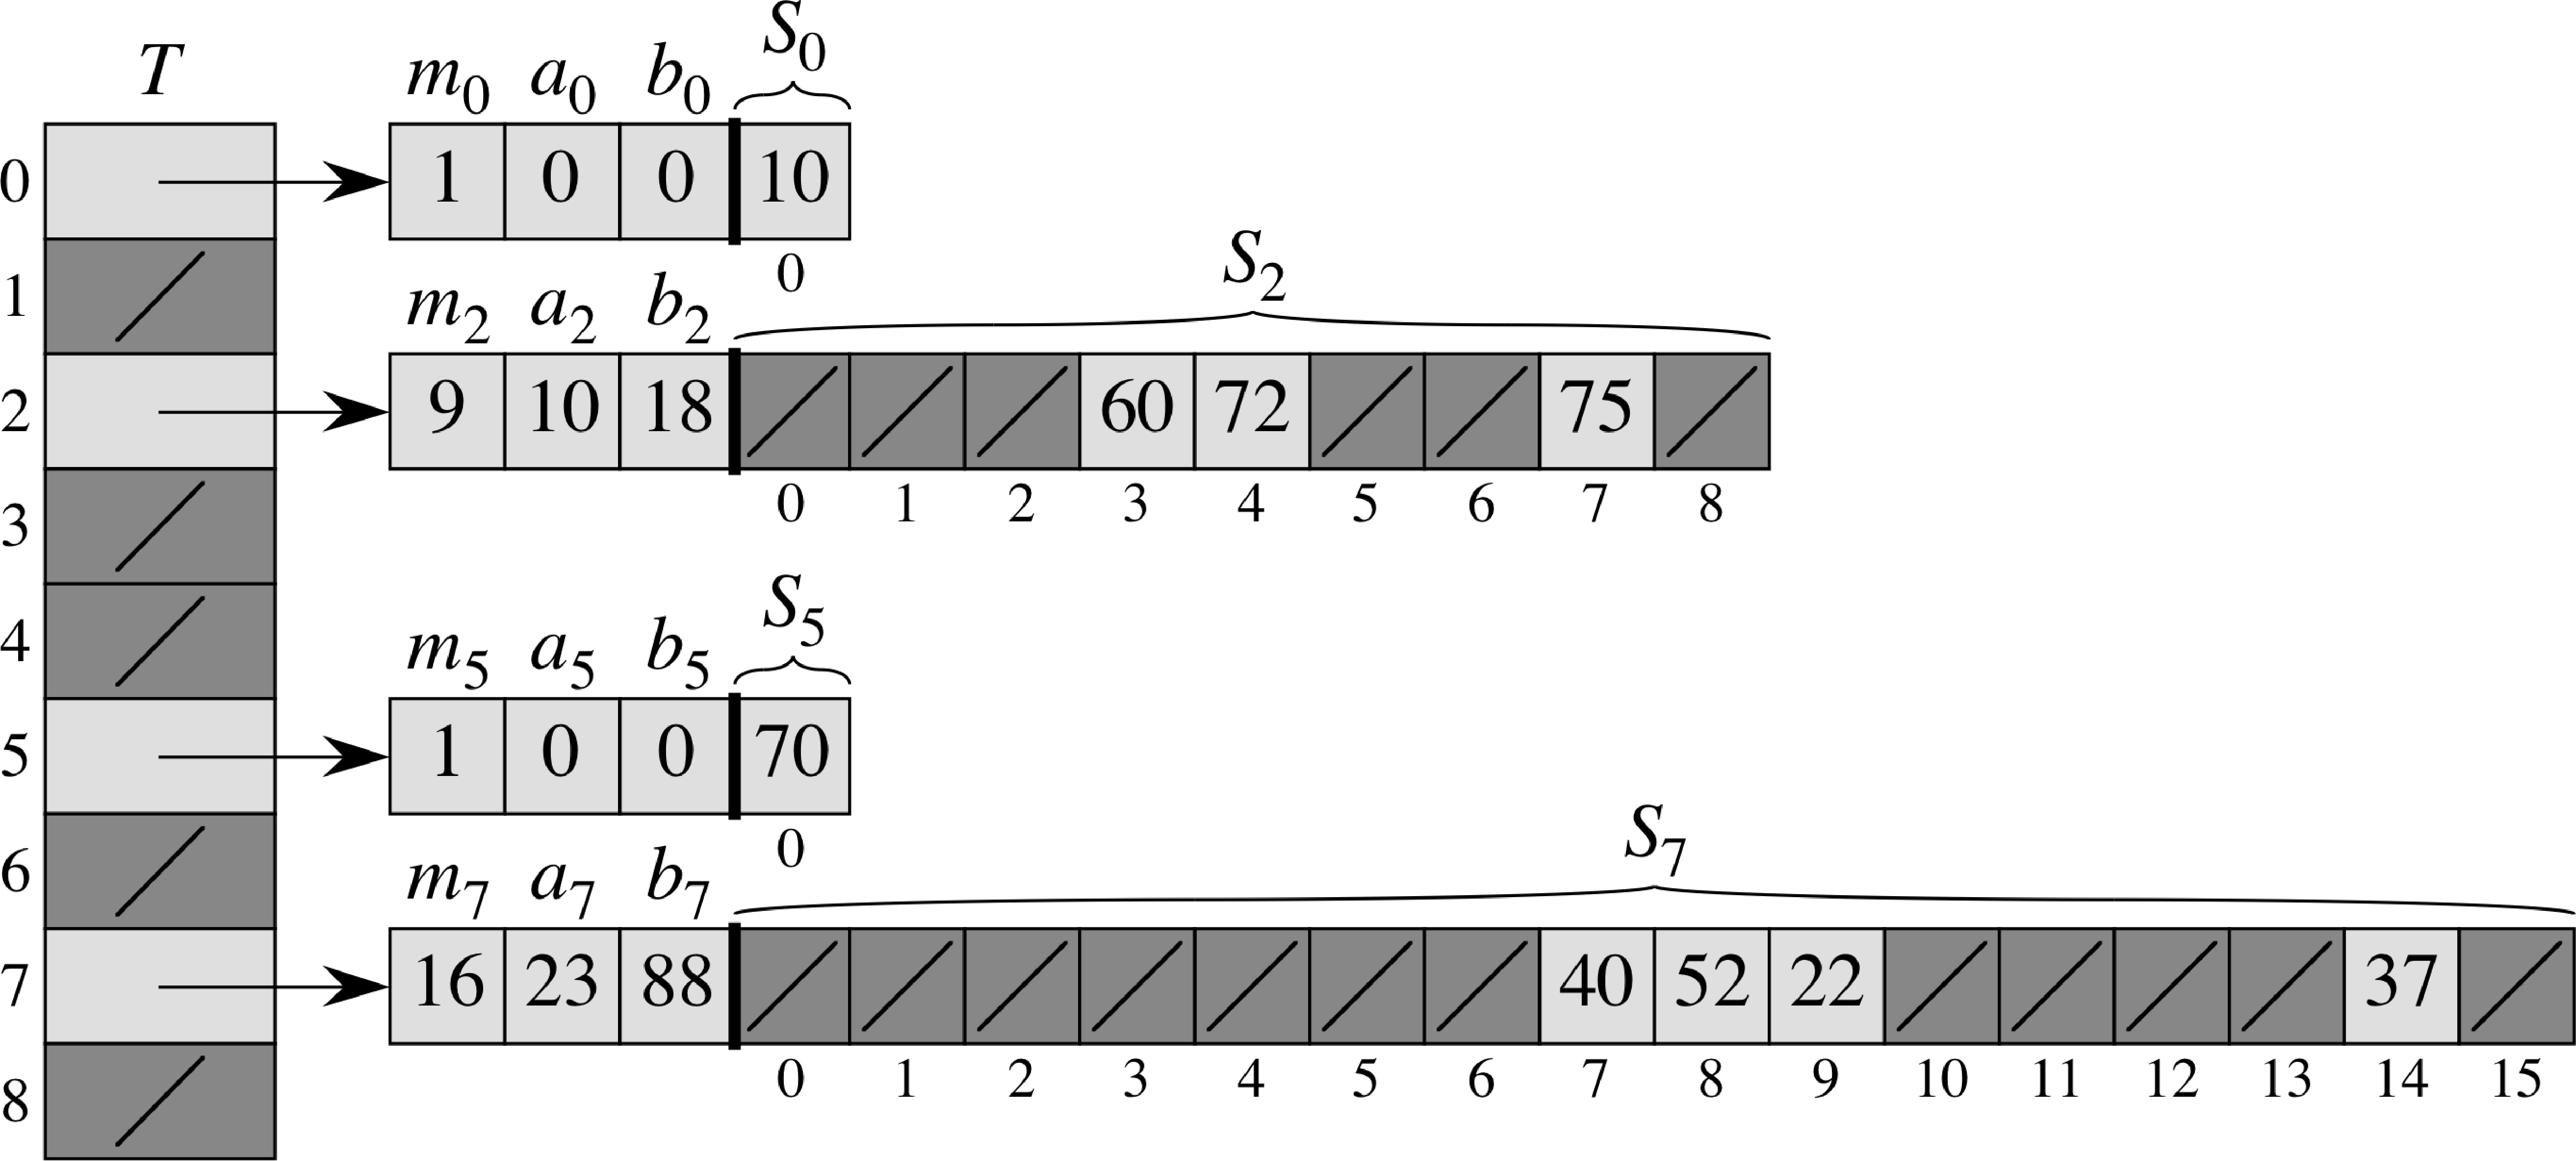
\includegraphics[width=\textwidth]{Fig-11-6.pdf}
\end{frame}



\end{document}
